\paragraph{} It is supposed to cost five years on my PhD program. Each year of the program comprises three semesters ($\approx$ 3 months), a summer vacation (3 months, always spent on internship or lab-work) and two short breaks (1 week). In the first two years of the program, I will take a number of courses required the program, and then I will have to take the qualification test for getting the master degree. Besides, I also have to put an eye on my research in the first two years, since Junfeng is going to obtain his tenure at the end of the second year. In the following years, the major task is going to be research, where two or more top conference publications (equivalent to two excellent projects) will be perfect for a successful graduate.

\paragraph{} During the fives years, I will have some long-term plans other than study and research, e.g., body building. Besides, I would also possibly have some short-term plans that deviate the default schedule. For example, I will try to get myself a chance to visit another lab for a view of research area. I also plan to spend one of the summer vacation on traveling or other personal purpose.

\paragraph{} In addition, the schedule is designed following some basic rules for flexibility and personal requirement.
\begin{itemize*}
\item Each day, sleeping should always cost 8 hours or more.
\item Each day, required working hours should never be more than 8 hours.
\item Timelines are always flexible.
\item Personal life should be an important piece in each day.
\end{itemize*}

\subsection{Semester}

In a semester, I have to focus on course study and research, while long-term plans should are not be left behind. Each workday starts at around 8am, and ends before 12am. The default plan is as following.

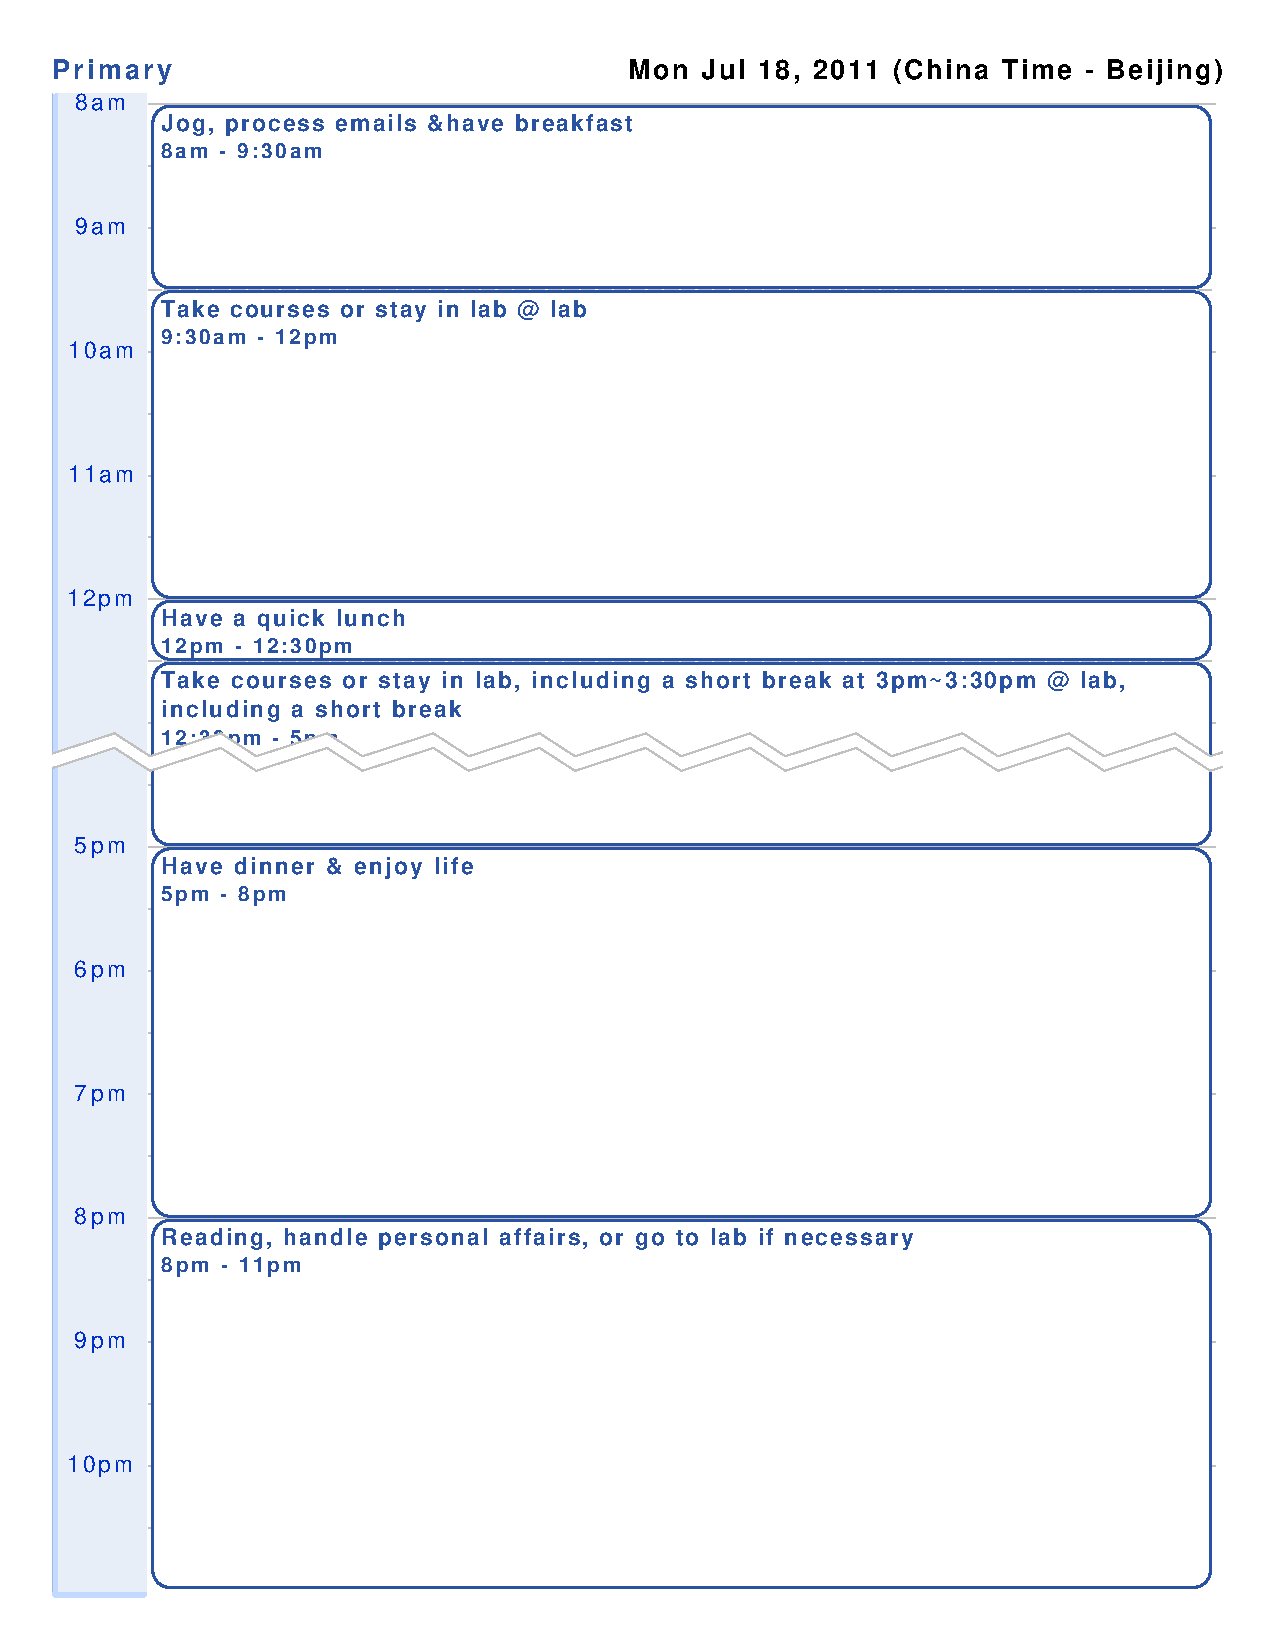
\includegraphics[width=0.95\textwidth]{figure/workday_semester.pdf}

Weekends are flexible.